\documentclass[a4paper,doc,natbib, floatsintext, hidelinks]{apa7}
\setcounter{secnumdepth}{3} % Add numbering to sections. 

\usepackage{authblk}
\usepackage[english]{babel}
\usepackage[utf8x]{inputenc}
\usepackage{amsmath}
\usepackage{graphicx}
\usepackage[colorinlistoftodos, textsize=scriptsize]{todonotes}

% Added by us
\usepackage{arydshln}
\usepackage{pdflscape}
\usepackage{cleveref}
\usepackage{xr}
\usepackage{caption}
\usepackage{lipsum}
\usepackage{float}
\usepackage{tikz}
\usepackage{tikz-qtree}
\usepackage{import}
\usepackage{lscape}
\usepackage{multicol}
\usepackage{makecell}
\usepackage{array}
\usepackage{color, colortbl}
\usepackage{xr}
%\externaldocument[supp-]{SM}
\newcolumntype{P}[1]{>{\centering\arraybackslash}m{#1}}
\newcommand{\YL}[1]{\textcolor{blue}{YL: #1}}
\newcommand{\YLDEL}[1]{\sout{\textcolor{black}{YL: #1}}}
\newcommand{\dieuwke}[1]{\textcolor{green!60!black}{DH: #1}}
\newcommand{\dnote}[1]{\todo[color=green!40, inline]{DH: #1}}
%
\renewrobustcmd{\bfseries}{\fontseries{b}\selectfont}
\renewrobustcmd{\boldmath}{}
\newrobustcmd{\B}{\bfseries}

\newcommand{\specialcell}[2][c]{\begin{tabular}[#1]{@{}l@{}}#2\end{tabular}}

\title{A Mechanism for Handling Nested Agreement Dependencies in Recurrent Neural Networks and Humans}
% \title{Exploring Processing of Nested Dependencies in Neural-Network Language Models and Humans}

% Exploring an Emergent Mechanism for Handling Nested Dependencies in a Recurrent Neural Network

% or A Mechanism for Handling Nested Agreement Dependencies in Recurrent Neural Networks and Humans

\shorttitle{Nested dependencies in NLMs and humans}

\sixauthors{Yair Lakretz}{Dieuwke Hupkes}{Alessandra Vergallito}{Marco Marelli}{Marco Baroni$^*$}{Stanislas Dehaene$^*$} 
\sixaffiliations{Cognitive Neuroimaging Unit, NeuroSpin center, 91191, Gif-sur-Yvette, France}{ILLC, University of Amsterdam, Amsterdam, Netherlands}{University of Milano-Bicocca, Milan, Italy}{University of Milano-Bicocca, Milan, Italy\\NeuroMI, Milan Center for Neuroscience, Milan, Italy}{Facebook AI Research, Paris, France\\Catalan Institute for Research and Advanced Studies, Barcelona, Spain, 08010\\Departament de Traduccio i Cencies del Llenguatge, Universitat Pompeu Fabra, Spain, 08018}{Cognitive Neuroimaging Unit, NeuroSpin center, 91191, Gif-sur-Yvette, France\\College de France, 11 Place Marcelin Berthelot, 75005 Paris, France} 


\begin{document}
\abstract{Recursive processing in sentence comprehension is considered a hallmark of human linguistic abilities. However, its underlying neural mechanism in the human brain remains largely unknown. Neural Language Models (NLMs) have recently shown remarkable success on various linguistic tasks. As the only non-human computational systems capable of accomplishing such tasks, NLMs offer new opportunities to study low-level mechanisms underlying natural language processing, which might give insights about human language processing. Here, we study syntactic processing in an NLM based on Recurrent Neural Networks with Long-Short Term Memory units. We use subject-verb number agreement as an index of syntactic processing in the NLM, and investigate the neural mechanisms underlying processing of nested agreement--a prototypical case of recursion. We find a small set of specialized units in the model that can successfully handle outermost agreements of nested constructions. An analysis of this mechanism predicts that, as it does not support full recursion, it will however run into trouble when processing embedded dependencies, especially if they are in turn long-range. We confirm this in simulations and further derive predictions about human performance based on the properties of the NLM agreement mechanism, which we test in a behavioral experiment. Unlike the NLM, humans do not exhibit a dramatic failure on embedded long-range dependencies. However, overall, human and NLM error patterns are remarkably similar, suggesting that exploring the ways in which NLMs process sentences might be a productive way to come up with precise hypotheses about human linguistic processing.}
% various effects in human data. We conclude that the NLM explains a large variance in human data, however, the network fails to find recursive processing of nested constructions.}

%We conclude by outlining future experiments that should establish whether the main discrepancy is quantitative (e.g., dependent on the number of nesting) or qualitative (e.g., due to recursive capabilities unique to humans).}
\keywords{Grammatical agreement, Long-Range Dependencies, Recursion, Recurrent Neural Networks, Language Models, Syntactic processing, Relative Clauses.}

\def\thefootnote{*}\footnotetext{Equal senior contribution.}

\maketitle
\import{sections/}{intro}
\import{sections/}{number_agreement_in_RNNs}
\import{sections/}{single_dependency_Italian}
\import{sections/}{two_dependencies}
\import{sections/}{discussion}

\bibliography{yair,marco,dieuwke}

\documentclass{article}

\usepackage{graphicx}
% \usepackage{cleveref}

\newcommand{\beginsupplement}{%
        \setcounter{table}{0}
        \renewcommand{\thetable}{S\arabic{table}}%
        \setcounter{figure}{0}
        \renewcommand{\thefigure}{S\arabic{figure}}%
     }

\begin{document}
\beginsupplement

\begin{figure*}
    \centering
    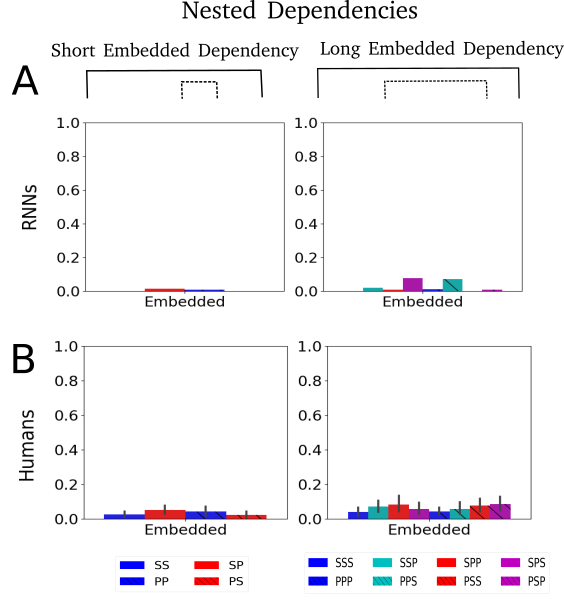
\includegraphics[width=10cm]{figures/error_rates_successive_all_conditions.png}
    \caption{\textbf{Error rates on Short- and Long-Successive:} collected from NLMs (panel A) and human subjects (B). Blue and red colors correspond to congruent and incongruent subjects, respectively. Secondary colors (cyan and magenta) indicate an attractor with an opposite number. Slant lines in bars indicate that the main subject is plural.}
    \label{fig:successive_all_conditions}
\end{figure*}
    
    
\begin{figure*}
    \centering
    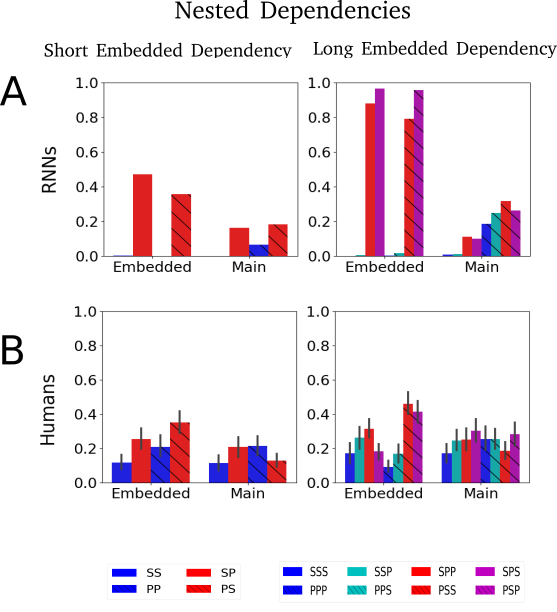
\includegraphics[width=10cm]{figures/error_rates_nested_all_conditions.png}
    \caption{\textbf{Error rates on Short- and Long-Nested:} collected from NLMs (panel A) and human subjects (B). Blue and red colors correspond to congruent and incongruent subjects, respectively. Secondary colors (cyan and magenta) indicate an attractor with an opposite number. Slant lines in bars indicate that the main subject is plural.}
    \label{fig:nested_all_conditions}
\end{figure*}
    
\end{document}


\end{document}
